\makeatletter
\def\input@path{{../}}
\makeatother
\documentclass[../master_thesis.tex]{subfiles}
\begin{document}
\chapter{Test Figures}\label{Figures}
\begin{figure}[hb!]
  \centering
  \begin{subfigure}[b]{0.75\linewidth}
    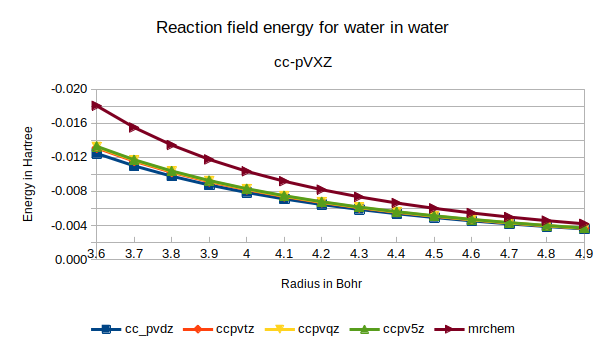
\includegraphics[width=\linewidth]{img/Erwat.png}
    \caption{\mrchem against normal basis sets}
  \end{subfigure}
  \begin{subfigure}[b]{0.75\linewidth}
    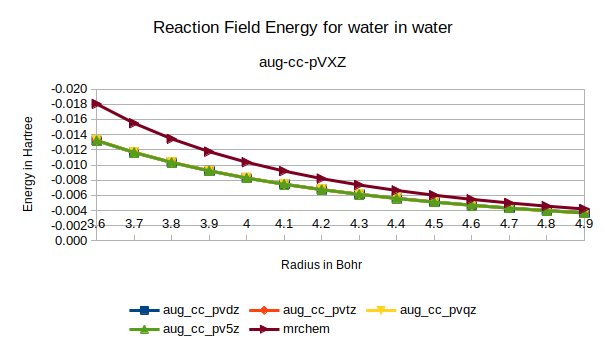
\includegraphics[width=\linewidth]{img/Eraugwat.png}
    \caption{\mrchem against augmented basis sets}
  \end{subfigure}
  \begin{subfigure}[b]{0.75\linewidth}
    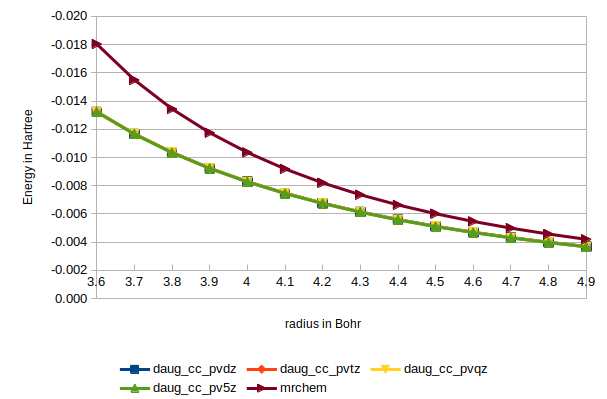
\includegraphics[width=\linewidth]{img/Erdaugwat.png}
    \caption{\mrchem against double augmented augmented basis sets}
  \end{subfigure}
  \caption[Reaction field energy of \ce{H_2O}]{Reaction field energy of \ce{H_2O} in a water solution, calculated with relative precision $e-05$ in \mrchem
  and with different basis sets in Gaussian}
  \label{fig:watEnergyplots}
\end{figure}

\begin{figure}[h!]
  \centering
  \begin{subfigure}[b]{0.75\linewidth}
    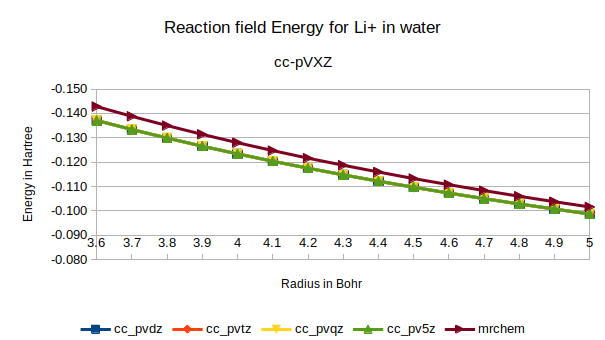
\includegraphics[width=\linewidth]{img/Erlip.png}
    \caption{\mrchem against normal basis sets}
  \end{subfigure}
  \begin{subfigure}[b]{0.75\linewidth}
    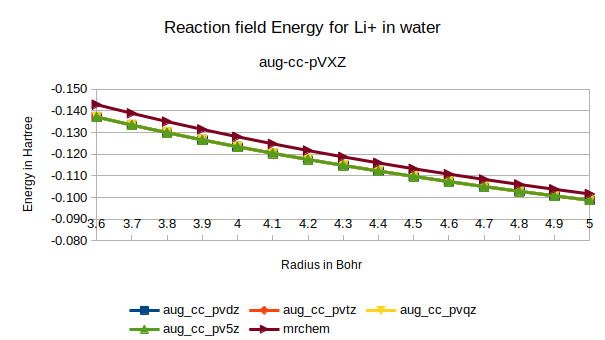
\includegraphics[width=\linewidth]{img/Erauglip.png}
    \caption{\mrchem against augmented basis sets}
  \end{subfigure}
  \begin{subfigure}[b]{0.75\linewidth}
    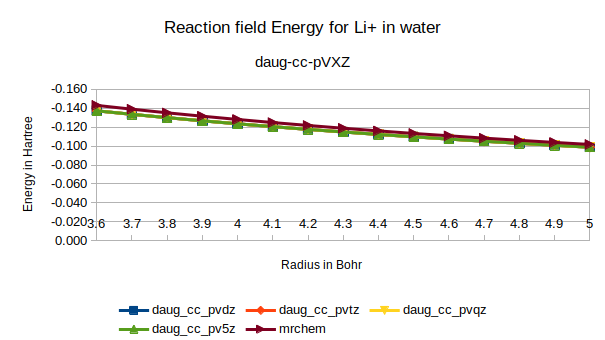
\includegraphics[width=\linewidth]{img/Erdauglip.png}
    \caption{\mrchem against double augmented augmented basis sets}
  \end{subfigure}
  \caption[Reaction field energy of \ce{Li^+}]{Reaction field energy of \ce{Li^+} in a water solution, calculated with relative precision $e-05$ in \mrchem
  and with different basis sets in Gaussian}
  \label{fig:lipEnergyplots}
\end{figure}

\begin{figure}[h!]
  \centering
  \begin{subfigure}[b]{0.75\linewidth}
    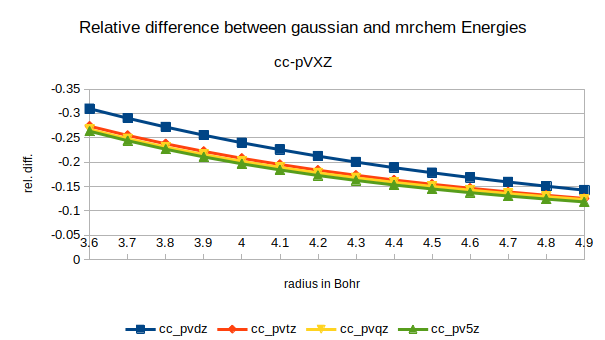
\includegraphics[width=\linewidth]{img/watreldiff.png}
    \caption{\mrchem against normal basis sets}
  \end{subfigure}
  \begin{subfigure}[b]{0.75\linewidth}
    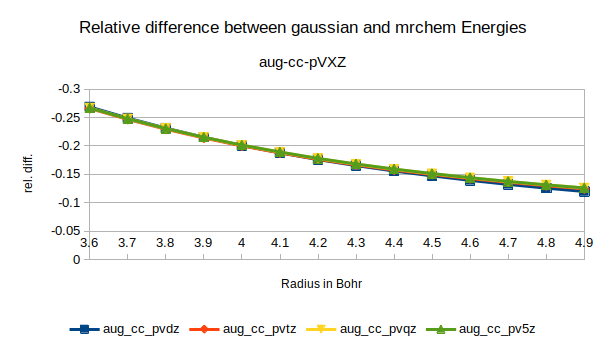
\includegraphics[width=\linewidth]{img/wataugreldiff.png}
    \caption{\mrchem against augmented basis sets}
  \end{subfigure}
  \begin{subfigure}[b]{0.75\linewidth}
    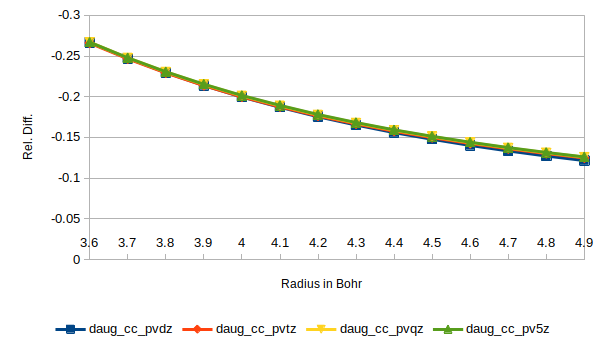
\includegraphics[width=\linewidth]{img/watdaugreldiff.png}
    \caption{\mrchem against double augmented augmented basis sets}
  \end{subfigure}
  \caption[Relative difference between methods for \ce{H_2O}]{Relative difference between the Reaction field energy of \ce{H_2O} in a water solution calculated with with relative precision $e-05$ in \mrchem
   and with different basis sets in Gaussian}
  \label{fig:watreldiffvar}
\end{figure}

\begin{figure}[h!]
  \centering
  \begin{subfigure}[b]{0.75\linewidth}
    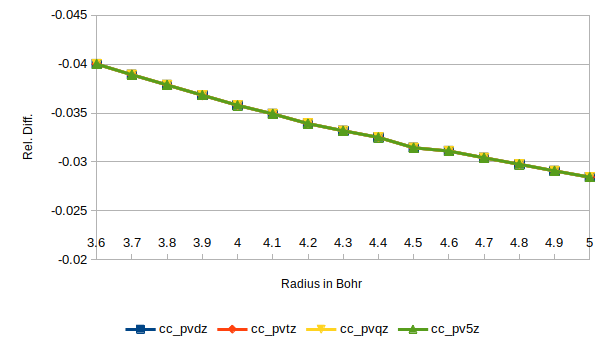
\includegraphics[width=\linewidth]{img/lipreldiff.png}
    \caption{\mrchem against normal basis sets}
  \end{subfigure}
  \begin{subfigure}[b]{0.75\linewidth}
    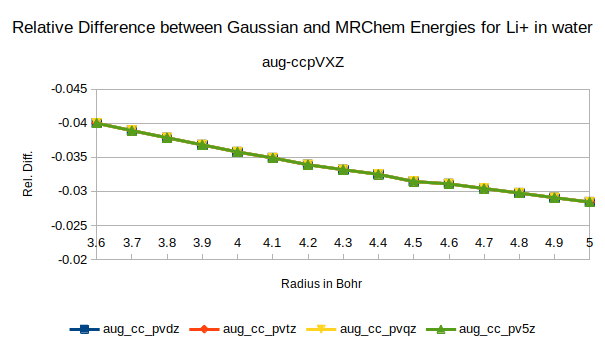
\includegraphics[width=\linewidth]{img/lipaugreldiff.png}
    \caption{\mrchem against augmented basis sets}
  \end{subfigure}
  \begin{subfigure}[b]{0.75\linewidth}
    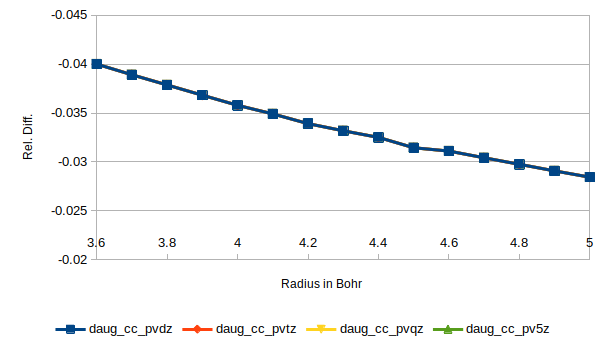
\includegraphics[width=\linewidth]{img/lipdaugreldiff.png}
    \caption{\mrchem against double augmented augmented basis sets}
  \end{subfigure}
  \caption[Relative difference between methods for \ce{Li^+}]{Relative difference between the Reaction field energy of\ce{Li^+} in a water solution calculated with relative precision $e-05$ in \mrchem
  and with different basis sets in Gaussian}
  \label{fig:lipreldiff}
\end{figure}

\begin{figure}[h!]
  \centering
  \begin{subfigure}[b]{0.75\linewidth}
    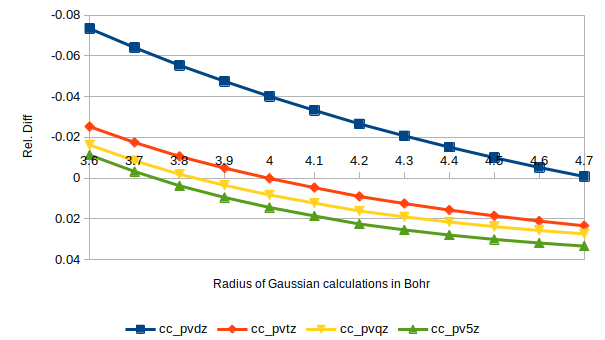
\includegraphics[width=\linewidth]{img/watreldiff02.png}
        \caption{\mrchem against normal basis sets}
  \end{subfigure}
  \begin{subfigure}[b]{0.75\linewidth}
    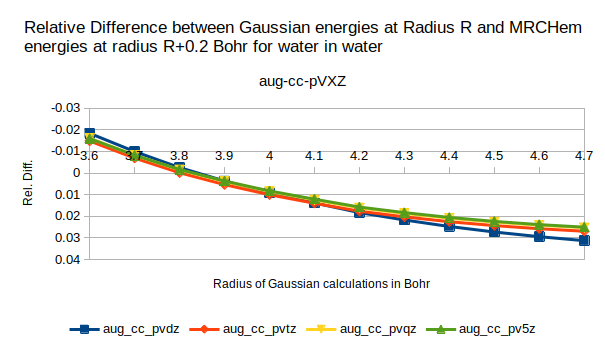
\includegraphics[width=\linewidth]{img/wataugreldiff02.png}
        \caption{\mrchem against augmented basis sets}
  \end{subfigure}
  \begin{subfigure}[b]{0.75\linewidth}
    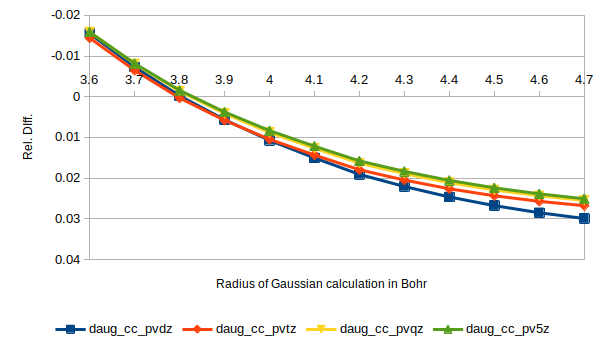
\includegraphics[width=\linewidth]{img/watdaugreldiff02.png}
    \caption{\mrchem against double augmented augmented basis sets}
  \end{subfigure}
  \caption[Relative difference between methods for \ce{H_2O} with radius $+0.2$ Bohr]{Relative difference between the Reaction field energy of \ce{H_2O}] with a shifted radius by $0.2$ Bohr in a water solution calculated with with relative precision $e-05$ in \mrchem
  and with different basis sets in Gaussian}
  \label{fig:watreldiff02}
\end{figure}

\begin{figure}[h!]
  \centering
  \begin{subfigure}[b]{0.75\linewidth}
    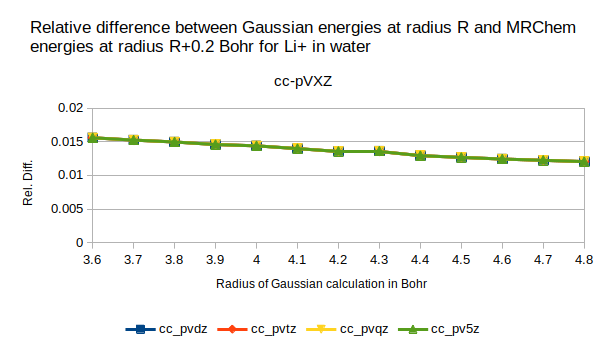
\includegraphics[width=\linewidth]{img/lipreldiff02.png}
    \caption{\mrchem against normal basis sets}
  \end{subfigure}
  \begin{subfigure}[b]{0.75\linewidth}
    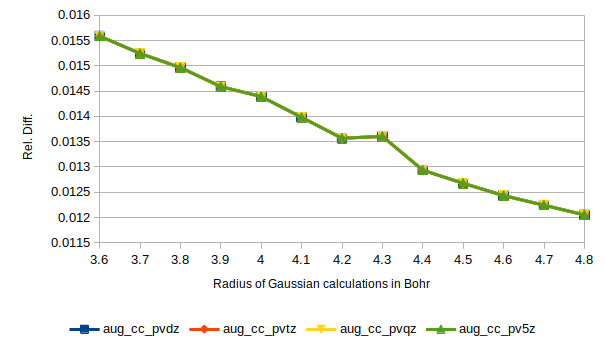
\includegraphics[width=\linewidth]{img/lipaugreldiff02.png}
    \caption{\mrchem against augmented basis sets}
  \end{subfigure}
  \begin{subfigure}[b]{0.75\linewidth}
    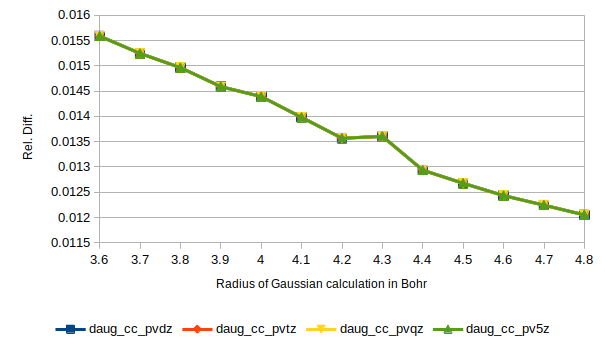
\includegraphics[width=\linewidth]{img/lipdaugreldiff02.png}
    \caption{\mrchem against double augmented augmented basis sets}
  \end{subfigure}
  \caption[Relative difference between methods for \ce{Li^+} with radius $+0.2$ Bohr]{Relative difference between the Reaction field energy of \ce{Li^+} with a shifted radius by $0.2$ Bohr in a water solution calculated with relative precision $e-05$ in \mrchem
  and with different basis sets in Gaussian}
  \label{fig:lipreldiff02}
\end{figure}

\begin{figure}[h!]
  \centering
  \begin{subfigure}[b]{0.75\linewidth}
    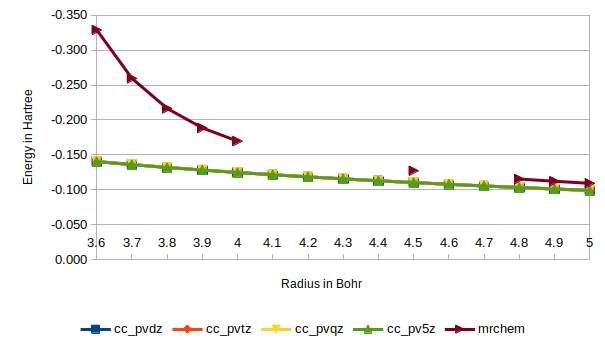
\includegraphics[width=\linewidth]{img/Ernop.png}
    \caption{\mrchem against normal basis sets}
  \end{subfigure}
  \begin{subfigure}[b]{0.75\linewidth}
    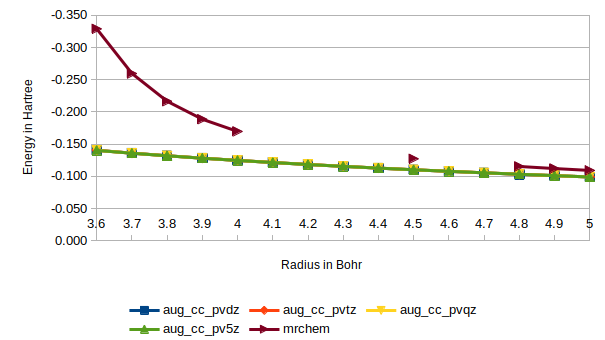
\includegraphics[width=\linewidth]{img/Eraugnop.png}
    \caption{\mrchem against augmented basis sets}
  \end{subfigure}
  \begin{subfigure}[b]{0.75\linewidth}
    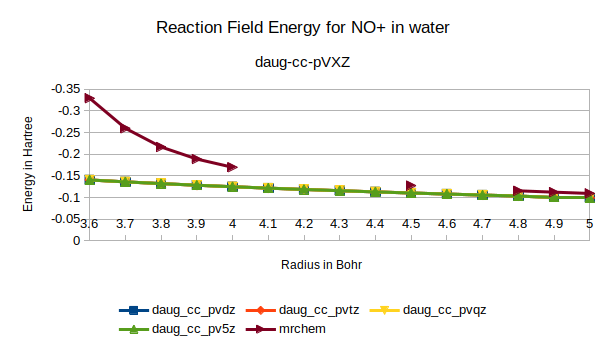
\includegraphics[width=\linewidth]{img/Erdaugnop.png}
    \caption{\mrchem against double augmented augmented basis sets}
  \end{subfigure}
  \caption[Energy plots for \ce{NO^+}]{Reaction field energy of \ce{NO^+} in a water solution, calculated with \mrchem
  and with different basis sets in Gaussian}
  \label{fig:nopEnergyplots}

\end{figure}
\begin{figure}[h!]
  \centering
  \begin{subfigure}[b]{0.75\linewidth}
    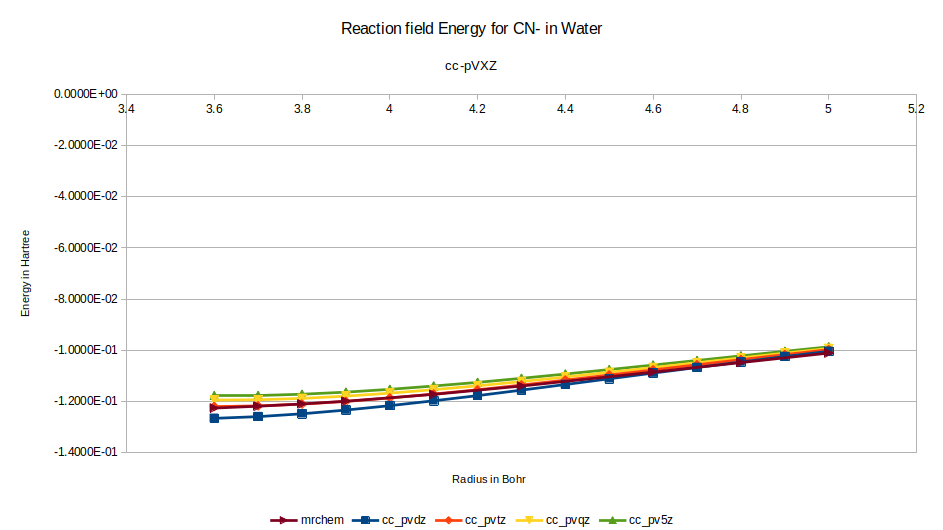
\includegraphics[width=\linewidth]{img/Ercyan.png}
    \caption{\mrchem against normal basis sets}
  \end{subfigure}
  \begin{subfigure}[b]{0.75\linewidth}
    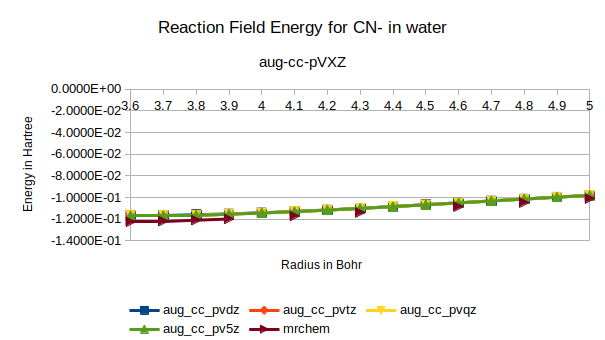
\includegraphics[width=\linewidth]{img/Eraugcyan.png}
      \caption{\mrchem against augmented basis sets}
  \end{subfigure}
  \begin{subfigure}[b]{0.75\linewidth}
    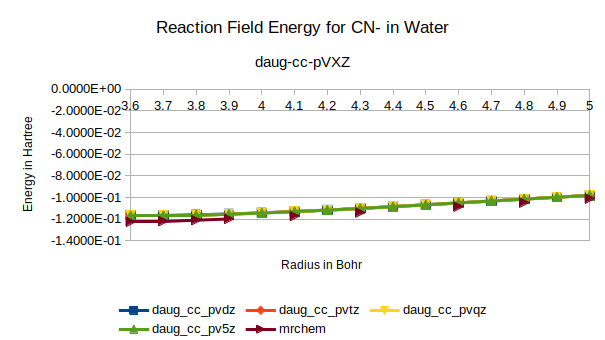
\includegraphics[width=\linewidth]{img/Erdaugcyan.png}
    \caption{\mrchem against double augmented augmented basis sets}
  \end{subfigure}
  \caption[Energy plots for \ce{CN^-}]{Reaction field energy of \ce{CN^-} in a water solution, calculated with \mrchem
  and with different basis sets in Gaussian}
  \label{fig:cyanEnergyplots}
\end{figure}

\begin{figure}[h!]
  \centering
  \begin{subfigure}[b]{0.75\linewidth}
    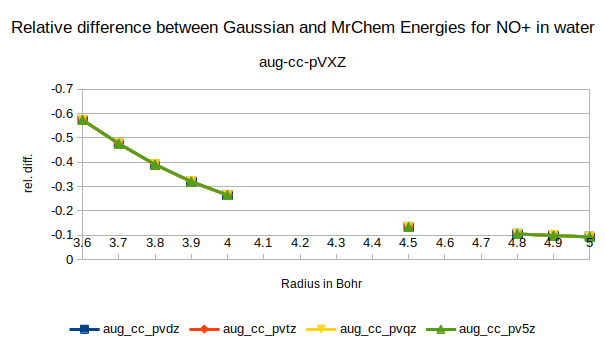
\includegraphics[width=\linewidth]{img/nopreldiff.png}
    \caption{\mrchem against normal basis sets}
  \end{subfigure}
  \begin{subfigure}[b]{0.75\linewidth}
    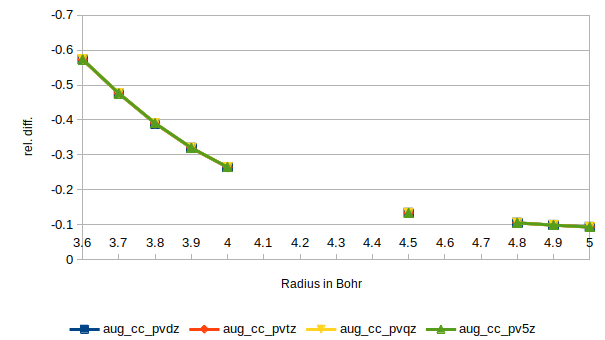
\includegraphics[width=\linewidth]{img/nopaugreldiff.png}
    \caption{\mrchem against augmented basis sets}
  \end{subfigure}
  \begin{subfigure}[b]{0.75\linewidth}
    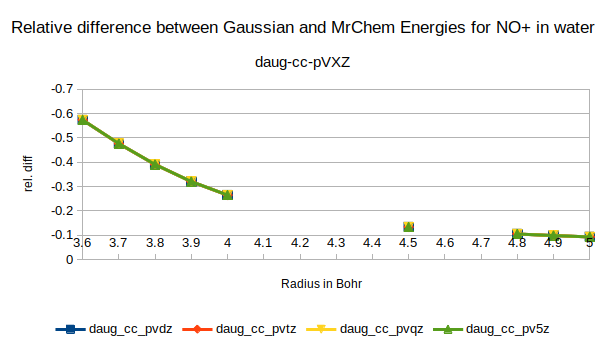
\includegraphics[width=\linewidth]{img/nopdaugreldiff.png}
    \caption{\mrchem against double augmented augmented basis sets}
  \end{subfigure}
  \caption[Relative difference between methods for \ce{NO^+}]{Relative difference between the Reaction field energy of \ce{NO^+} in a water solution calculated with \mrchem
  and with different basis sets in Gaussian}
  \label{fig:nopreldiff}
\end{figure}

\begin{figure}[h!]
  \centering
  \begin{subfigure}[b]{0.75\linewidth}
    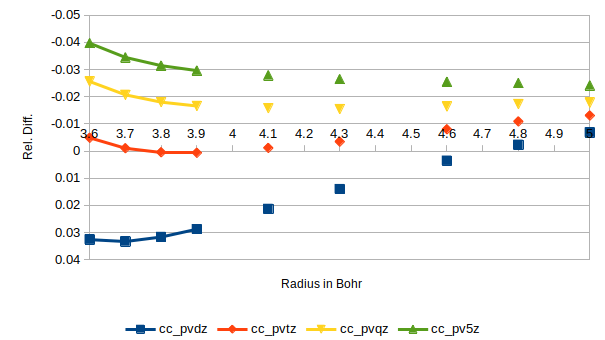
\includegraphics[width=\linewidth]{img/cyanreldiff.png}
    \caption{\mrchem against normal basis sets}
  \end{subfigure}
  \begin{subfigure}[b]{0.75\linewidth}
    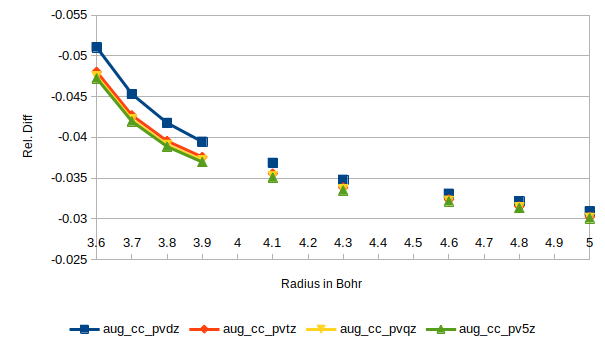
\includegraphics[width=\linewidth]{img/cyanaugreldiff.png}
    \caption{\mrchem against augmented basis sets}
  \end{subfigure}
  \begin{subfigure}[b]{0.75\linewidth}
    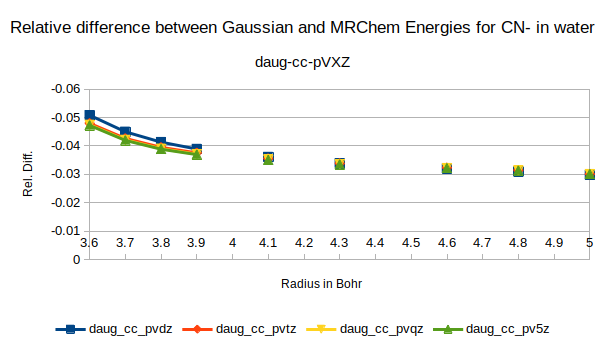
\includegraphics[width=\linewidth]{img/cyandaugreldiff.png}
    \caption{\mrchem against double augmented augmented basis sets}
  \end{subfigure}
  \caption[Relative difference between methods for \ce{CN^-}]{Relative difference between the Reaction field energy of \ce{CN^-} in a water solution calculated with \mrchem
  and with different basis sets in Gaussian}
  \label{fig:cyanreldiff}
\end{figure}


\begin{acronym}
\acro{AUS}[\href{https://www.sigma2.no/content/advanced-user-support}{AUS}]{Numerical Methods in Quantum Chemistry}
\acro{BO}{Born-Oppenheimer}
\acro{CTCC}[\href{http://www.ctcc.no}{CTCC}]{Centre for Theoretical and Computational Chemistry}
\acro{DC}{Dielectric Continuum}
\acro{DFT}{Density Functional Theory}
\acro{EFP}{Effective Fragment Potential}
\acro{EU}{European Union}
\acro{HF}{Hartree-Fock}
\acro{Hylleraas}[\href{https://www.mn.uio.no/hylleraas/english/}{Hylleraas}]{Hylleraas
  Centre for Quantum Molecular Sciences}
\acro{HPC}{High Performance Computing}
\acro{KTH}{Royal Institute of Technology}
\acro{LDA}{Local Density Approximation}
\acro{MCD}{Magnetic Circular Dichroism}
\acro{MCSCF}{Multiconfiguration Self Consistent Field}
\acro{MM}{Molecular Mechanics}
\acro{MW}{Multiwavelet}
\acro{NFR}{Norwegian Research Council}
\acro{NMQC}[\href{http://www.ctcc.no/events/conferences/2015/numeric-conference/}{NMQC}]{Numerical Methods in Quantum Chemistry}
\acro{NOTUR}[\href{https://www.notur.no/}{NOTUR}]{Norwegian Metacenter for Computational Science}
\acro{PCM}{Polarizable Continuum Model}
\acro{PI}{Primcipal Investigator}
\acro{QC}{Quantum Chemistry}
\acro{QM}{Quantum Mechanics}
\acro{QM/MM}{Quantum Mechanics/Molecular Mechanics}
\acro{ROA}{Raman Optical Activity}
\acro{SC}{semiconductor}
\acro{SCF}{Self Consistent Field}
\acro{SHG}{Second Harmonic Genertation}
\acro{STSM}{Short-term scientific mission}
\acro{TPA}{Two-Photon Absorption}
\acro{WP}{Work Package}
\acro{CBS}{Complete Basis Set}
\acro{TCG}{Theoretical Chemistry Group}
\acro{vdW}{van der Waals}
\acro{SE}{Schrödinger Equation}
\acro{PES}{Potential Energy Surface}
\acro{LCAO}{Linear Combination of Atomic Orbitals}
\acro{MRA}{Multi-Resolution Analysis}
\acro{NS}{Nonstandard}
\end{acronym}

\biblio
\end{document}
